%% LyX 2.2.2 created this file.  For more info, see http://www.lyx.org/.
%% Do not edit unless you really know what you are doing.
\documentclass[english]{article}
\usepackage[T1]{fontenc}
\usepackage[latin9]{inputenc}
\usepackage{float}
\usepackage{graphicx}
\usepackage{babel}
\begin{document}

\subsection{Anexo - Ejercicio 3 - Mediciones de las oscilaci�nes}

Se procedi� a intentar obtener evidencia experimental sobre las oscilaciones
del circuito (colocando el valor de $R5$ con los valores que en la
simulaci�n provocaron oscilaciones). Debido a que la frecuencia de
dichas oscilaciones fue m�s alta que lo esperado $>20Mhz$ se debi�
conectar a la entrada de una se�al de muy alta frecuencia (del orden
de 20Mhz) para lograr que el periodo de oscilaci�n fuese comparable
con el periodo de la se�al de salida. Se muestran a continuaci�n algunas
imagenes obtenidas donde hay evidencia importante de la oscilaci�n
de la salida.

\begin{figure}[H]
\begin{centering}
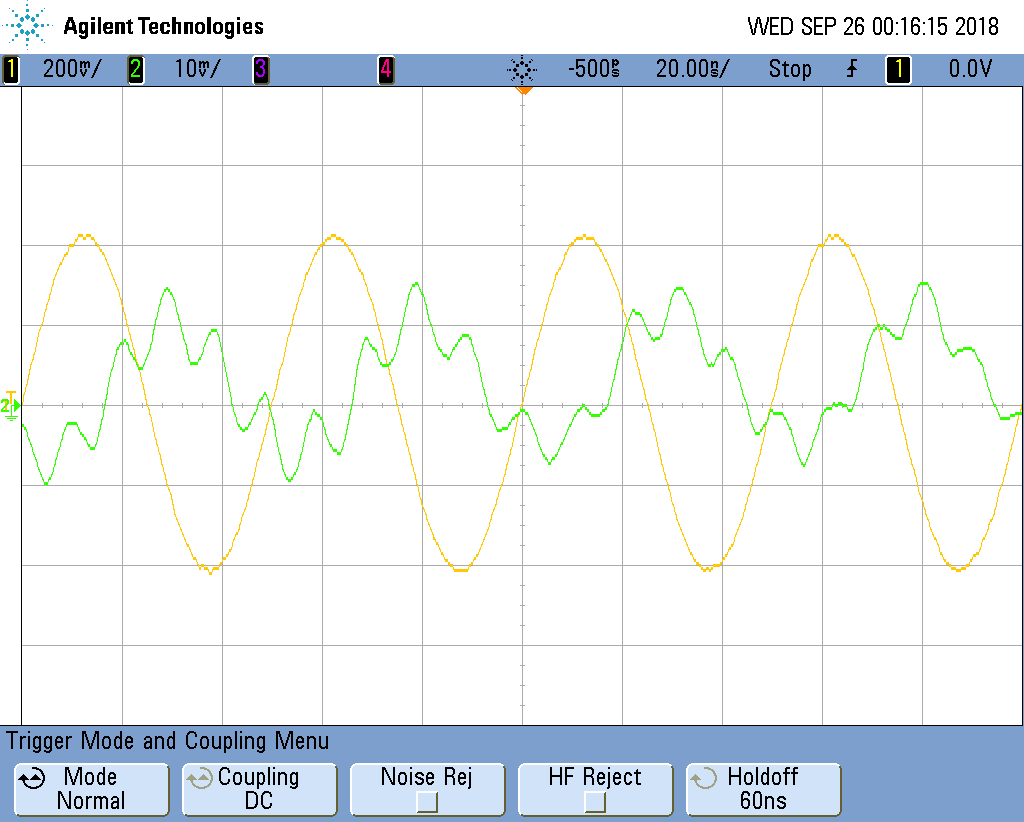
\includegraphics[scale=0.5]{osciloscopio/oscila3}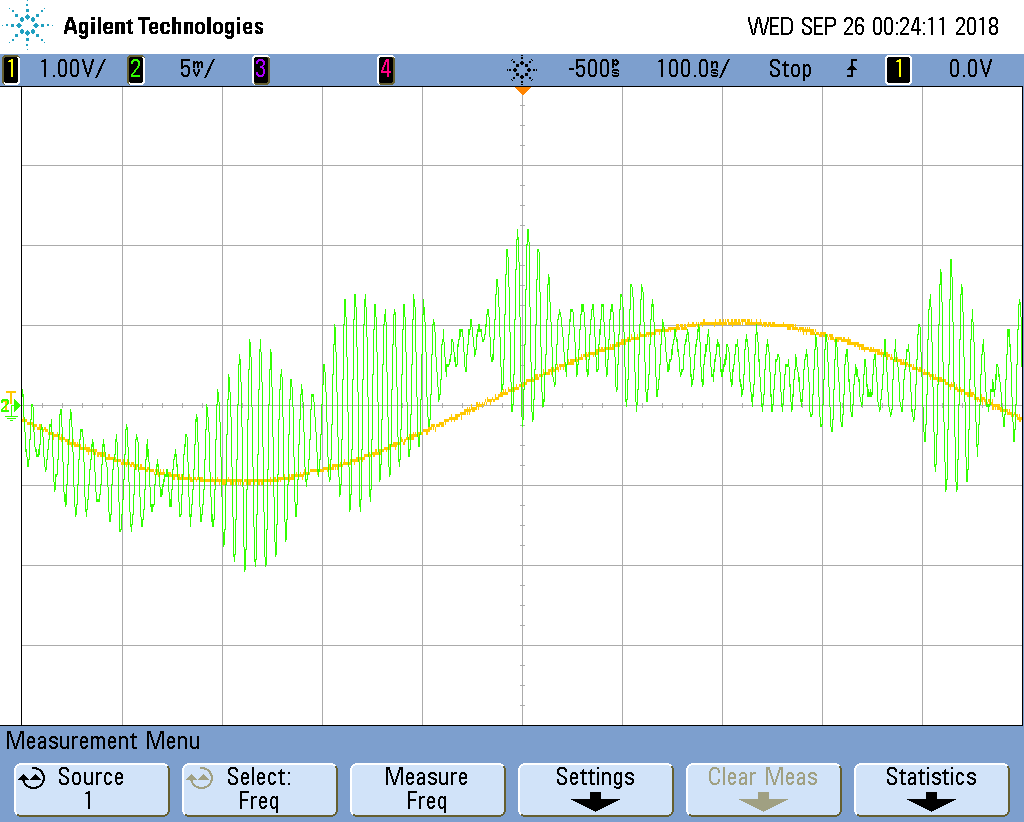
\includegraphics[scale=0.2]{osciloscopio/oscila5}
\par\end{centering}
\caption{Evidencia acerca de la oscilaci�n de la se�al de salida - modo com�n
- frecuencias $20Mhz$ y $1Mhz$}
\end{figure}

Es importante notar que para poder notar el efecto de las oscilaciones
en el osciloscopio se debi� colocar el circuito en frecuencias fuera
del rango de operaci�n del amplificador; no fueron se�ales faciles
de medir, pero, es un hecho que el circuito dej� de funcionar tanto
en bajas como altas frecuencias al colocar el valor de $R_5 < 8k$,
por lo que la hiotesis es que a pesar de dichas oscilaciones ser de
alta frecuencia, provocan de todas formas un incorrecto funcionamiento
del circuito.
\end{document}
